%\documentclass[10pt,twoside,a4paper]{report}
\documentclass[10pt,a4paper]{report}

\usepackage[latin1]{inputenc}
\usepackage[english]{babel}
\usepackage{enumerate}
\usepackage{amsmath}
\usepackage{amssymb}
\usepackage{amsthm}
\usepackage{latexsym}
\usepackage{makeidx}
%\usepackage{showidx}
\usepackage[retainorgcmds]{IEEEtrantools}

\makeindex

% --------------------------------------------------------------------- Symbols
\renewcommand{\phi}{\varphi}
\newcommand{\Cayley}{\Psi}
\newcommand{\ModCayley}{\Phi}

% ------------------------------------------------------------------------ Sets
\newcommand{\N}{\mathbb{N}}
\newcommand{\R}{\mathbb{R}}
\newcommand{\Q}{\mathbb{Q}}
\newcommand{\Irrat}{\mathbb{I}}
\newcommand{\Rplus}{\R^{+}}
\newcommand{\C}{\mathbb{C}}
\newcommand{\Z}{\mathbb{Z}}
\newcommand{\EC}{\C_{\infty}}
\newcommand{\EQ}{\Q_{\infty}}
%\newcommand{\RS}{\mathcal{S}}
\newcommand{\UnitCirc}{S^{1}}
\newcommand{\UnitSphere}{S_1}
\newcommand{\EU}{\mathcal{H}^\ast}

\newcommand{\Syms}{\Sigma}
\newcommand{\Words}[1]{{#1}^{\star}}
\newcommand{\FunDom}{\mathcal{F}}
\newcommand{\FunSet}{\mathcal{F}^\ast}
\newcommand{\Indisk}{\mathcal{I}}

\newcommand{\presentation}[2]{\left\langle #1 \mid #2 \right\rangle}
\newcommand{\FreeGrp}[1]{{#1}_{\sim}}

\newcommand{\LinGrp}[3]{\operatorname{#1}_{#2}(#3)}

\newcommand{\GLn}[2]{\LinGrp{GL}{#1}{#2}}
\newcommand{\SLn}[2]{\LinGrp{SL}{#1}{#2}}
\newcommand{\PGLn}[2]{\LinGrp{PGL}{#1}{#2}}
\newcommand{\PSLn}[2]{\LinGrp{PSL}{#1}{#2}}

\newcommand{\GL}[1]{\GLn{2}{#1}}
\newcommand{\SL}[1]{\SLn{2}{#1}}
\newcommand{\PGL}[1]{\PGLn{2}{#1}}
\newcommand{\PSL}[1]{\PSLn{2}{#1}}

\newcommand{\Stabilizer}[2]{{#1}_{#2}}

\newcommand{\Center}[1]{\operatorname{Z}(#1)}

\newcommand{\Mat}[3]{{#1}^{#2 \times #3}}
\newcommand{\SqMat}[2]{\Mat{#1}{#2}{#2}}

\newcommand{\ModGrp}{\Gamma}

\newcommand{\setdefsz}[3]{#1\{ #2 \ #1| \ #3 #1\}}
\newcommand{\setdef}[2]{\setdefsz{}{#1}{#2}}

\newcommand{\fundef}[5]{#1 : \left\{
\begin{matrix} 
#2 &\to& #3 \\ 
#4 &\mapsto& #5
\end{matrix}
\right.}

% ------------------------------------------------------------------ References
\newcommand{\Schoeneberg}{Schoeneberg~\cite{schoeneberg1974elliptic}}
\newcommand{\Klein}{Klein/Fricke~\cite{klein1966vorlesungen}}
\newcommand{\Hungerford}{Hungerford~\cite{hungerford1974algebra}}
\newcommand{\Lehner}{Lehner~\cite{lehner1982discontinuous}}

% ---------------------------------------------------------------------- Macros
\newcommand{\todo}[2]{\bigskip\noindent\framebox[\textwidth]{\emph{TODO #1:} #2}\bigskip}

% --------------------------------------------------------------- Abbreviations
\newcommand{\ie}{i.e.\ }
\newcommand{\eg}{e.g.\ }
\newcommand{\resp}{resp.\ }
\newcommand{\Wlog}{W.l.o.g.\ }

% ------------------------------------------------------------------- Functions
\newcommand{\lxor}{\overset{.}{\lor}}

\newcommand{\floor}[1]{\left\lfloor #1 \right\rfloor}
\newcommand{\ceil}[1]{\left\lceil #1 \right\rceil}
\newcommand{\nint}[1]{\operatorname{nint}\left( #1 \right)}
\newcommand{\sgn}[1]{\operatorname{sgn}\left( #1 \right)}

\newcommand{\topcl}[1]{\operatorname{cl}(#1)}

\newcommand{\half}[1]{\frac{#1}{2}}
\newcommand{\reci}[1]{\frac{1}{#1}}

\newcommand{\cfr}[2]{
\begin{array}{c}\multicolumn{1}{c|}{#1}\\
\hline\multicolumn{1}{|c}{#2}\end{array}}

\newcommand{\inv}[1]{{#1}^{-1}}

\newcommand{\moebius}[5]{\frac{#1 #5 + #2}{#3 #5 + #4}}
\newcommand{\mat}[4]{\begin{pmatrix}#1 & #2 \\ #3 & #4\end{pmatrix}}
\newcommand{\smallmat}[4]{\left({}^{#1}_{#3}\ {}^{#2}_{#4}\right)}
\newcommand{\rvec}[2]{\begin{pmatrix}#1 & #2\end{pmatrix}}
\newcommand{\cvec}[2]{\begin{pmatrix}#1 \\ #2\end{pmatrix}}
\newcommand{\transp}[1]{#1^{\textrm{T}}}
\newcommand{\htransp}[1]{#1^{\textrm{H}}}
\newcommand{\id}[1]{\operatorname{id}_{#1}}

\newcommand{\abs}[1]{\left|#1\right|}
\newcommand{\conj}[1]{\overline{#1}}
\renewcommand{\Re}[1]{\operatorname{Re}\left(#1\right)}
\renewcommand{\Im}[1]{\operatorname{Im}\left(#1\right)}

\newcommand{\epo}[1]{e^{#1}}
\newcommand{\ii}{i}

\newcommand{\eucnorm}[1]{\left\| #1 \right\|_2}

% ---------------------------------------------------------------- Environments

\newtheorem{theorem}{Theorem}[chapter]
\newtheorem{corollary}[theorem]{Corollary}
\newtheorem{lemma}[theorem]{Lemma}

\theoremstyle{definition}
\newtheorem{definition}[theorem]{Definition}
\newtheorem{example}[theorem]{Example}

\theoremstyle{remark}
\newtheorem{remark}[theorem]{Remark}


\title{Computer Algebra and Analysis:\\Complex Variables Visualized}
\author{Thomas Ponweiser}
\date{\today}

\begin{document}

\maketitle

\pagestyle{headings}

\tableofcontents

% ------------------------------------------------------- CHAPTER: INTRODUCTION
\chapter{Introduction}

% -------------------------------------------- Section: Algebraic constructions
\section{Groups and basic algebraic constructions}

In this section, we recapitulate some basic algebraic concepts, most important the notions of \emph{free groups} and \emph{free products}, and the construction of a group in terms of \emph{generators} and \emph{relations}. 

\subsection{Free monoids}
\index{Free!monoid}
Let $\Sigma$ be a set of formal symbols, for example $\Sigma = \{a, b, c, \dots\}$. Then, the set of words over the alphabet $\Sigma$ is defined as
\begin{equation}
\label{eqn_SigmaStarDef}
\Words{\Sigma} := \bigcup_{n\ge0} \Sigma^n.
\end{equation}
We will call the elements of $\Words{\Sigma}$ \emph{words}. To make things easier, we will omit the parentheses when notating such a word $w \in \Words{\Sigma}$, e.g. $w = (a,b,b,a) =: abba$. Note, that also the empty tuple, which we will call the \emph{empty word} and denote as $\epsilon$, is an element of $\Words{\Sigma}$. It is now just natural to define a binary operation $\cdot$ on $\Words{\Sigma}$ which is given by concatenation of words:
\begin{equation*}
w_1 \cdot w_2 = w_1 w_2, \quad w_1, w_2 \in \Words{\Sigma}.
\end{equation*}
Obviously, $\Words{\Sigma}$ is closed under this operation and $\epsilon$ is a the neutral element. Thus $\Words{\Sigma}$ together with the operation $\cdot$ forms a monoid. Note, that in the exceptional case, when $\Sigma = \emptyset$ and thus $\Words{\Sigma} = \{\epsilon\}$, we obtain the trivial monoid by this construction. 

\begin{definition}
\label{dfn_FreeMonoid}
Let $\Sigma$ be an arbitrary set of symbols (called the alphabet), and $\Words{\Sigma}$ be defined as in (\ref{eqn_SigmaStarDef}). Moreover, denote concatenation of words by $\cdot$ and let $\epsilon$ be the empty word. Then, the algebraic structure $\langle \Words{\Sigma}, \cdot, \epsilon \rangle$ is called the \emph{free monoid over the alphabet $\Sigma$}.
\end{definition} 

\subsection{Free groups}
\index{Free!group}
In a similar fashion, we can construct also a group from any given formal alphabet $\Sigma$. For this purpose we first choose a disjoint copy of $\Sigma$, denoted by $\inv{\Sigma}$, and a bijection $f : \Sigma \to \inv{\Sigma}$. We can extend this bijection between the sets $\Sigma$ and $\inv{\Sigma}$ to an involution on their union $\overline{\Sigma} := (\Sigma \cup \inv{\Sigma})$ by simply defining $f(f(a)) := a$ for all $a \in \Sigma$. Now we introduce the notation $f(a) =: \inv{a}$ and call $\inv{a}$ the \emph{(formal) inverse} of the symbol $a \in \overline{\Sigma}$.

\index{Reduced form}
Next, we construct the free monoid $\Words{\overline{\Sigma}}$. If $\sigma_1, \sigma_2, \dots, \sigma_n$ are symbols of $\overline{\Sigma}$, then we say the word $\sigma_1 \sigma_2 \dots \sigma_n$ is \emph{reduced}, if and only if no two subsequent symbols of the word are inverse to each other, that is
\begin{equation}
\label{eqn_GrpWordReducedForm}
 \sigma_j \ne \sigma_{j+1}^{-1} \quad \text{for all } 1 \le j < n.
\end{equation}
Clearly, every word $w \in \Words{\overline{\Sigma}}$ can be brought into reduced form by successively ``canceling out'' adjacent inverse symbols until finally a word is obtained, which satisfies (\ref{eqn_GrpWordReducedForm}). We call the result of this procedure the \emph{reduced form of $w$}. Additionally, we define two words $w_1, w_2 \in \Words{\overline{\Sigma}}$ to be \emph{equivalent}, if and only if they have the same reduced form and we write $w_1 \sim w_2$ in this case. It is easy to see that this relation is a congruence relation (i.e. is compatible with word-concatenation)\footnote{Denote the reduced form of a word $w$ as $\phi(w)$. If $w_1 \sim w_2$ and $v_1 \sim v_2$ are given, then we also have $w_1 v_1 \sim w_2 v_2$ because $\phi(w_1) = \phi(w_2) := w$ and $\phi(v_1) = \phi(v_2) := v$ implies $\phi(w_1 v_1) = \phi(w v) = \phi(w_2 v_2)$.} and thus we can consider also the set of equivalence classes $\Words{\overline{\Sigma}}/_{\sim}$ as monoid under the operation of word-concatenation. Obviously the set of reduced words is a representative system for $\Words{\overline{\Sigma}}/_{\sim}$ and we agree to denote an equivalence class $[w]_{\sim}$ simply by the reduced word $w$. $\Words{\overline{\Sigma}}/_{\sim}$ is not just a monoid, but in fact a group, as the inverse of a word $\sigma_1 \sigma_2 \dots \sigma_{n-1} \sigma_n$ is trivially given by $\sigma_n^{-1} \sigma_{n-1}^{-1} \dots \sigma_2^{-1} \sigma_1^{-1}$. 
\begin{definition}
\label{dfn_FreeGroup}
Let $\Sigma$ be an arbitrary set of formal symbols and define $\overline{\Sigma} := \Sigma \cup \inv{\Sigma}$ as above. On the free monoid $\Words{\overline{\Sigma}}$ define an equivalence relation $\sim$ by identifying words with same reduced form. Then, the algebraic structure $\langle \Words{\overline{\Sigma}}/_{\sim}, \cdot, \epsilon \rangle$ is called the \emph{free group over the alphabet $\Sigma$}.
\end{definition}
\begin{remark}
In the exceptional case, when $\Sigma = \emptyset$  we obtain the trivial group by this construction\footnote{If $\Sigma = \emptyset$ then we can also choose $\inv{\Sigma} = \emptyset$ ($\Sigma$ and $\inv{\Sigma}$ are then disjoint as required). It follows that also $\overline{\Sigma}$ is empty and we end up with the trivial monoid $\{\epsilon\}$, which is in the same time the trivial group.}.
\end{remark}


% --------------------------------------------- Section: M�bius transformations
\section{M�bius transformations}

In the following we define the group of M�bius transformations and collect some useful basic properties.

\begin{definition}
\label{dfn_MoebiusTransform}
\index{Mobius transformation@M�bius transformation}
A non-constant rational function $\phi \in \C(z)$ of the form 
\begin{equation*}
\phi(z) = \moebius{a}{b}{c}{d}{z},\quad a, b, c, d \in \C,\quad ad - bc \ne 0
\end{equation*}
is called \emph{M�bius transformation}.
\end{definition}

\begin{remark}
The condition $ad - bc \ne 0$ just ensures that $\phi$ is in fact non-constant.
\end{remark}

\begin{theorem}
\label{thm_MoebiusGroup}
The set of M�bius transformations forms a group under the action of function composition and can be identified with the projective general linear group $\PGL{\C}$ or the projective special linear group $\PSL{\C}$.
\end{theorem}
\begin{proof}
Let $\phi$ and $\psi$ be M�bius transformations with
\begin{equation*}
\phi(z) = \moebius{a}{b}{c}{d}{z},\quad \psi(z) = \moebius{e}{f}{g}{h}{z}.
\end{equation*}

First, we make the trivial observation, that composing those two transformations again yields a rational function of the desired form:
\begin{equation}
\label{eqn_MoebiusComposition}
\phi \circ \psi(z) 
 = \moebius{a}{b}{c}{d}{\moebius{e}{f}{g}{h}{z}} 
 = \frac{aez + af + bgz + bh}{cez + cf + dgz + dh} 
 = \moebius{(ae + bg)}{(af + bh)}{(ce + dg)}{(cf + dh)}{z}
\end{equation}

Having a closer look on the resulting coefficients one might notice that they relate to the following matrix product:
\begin{equation}
\label{eqn_MatrixProduct}
\mat{a}{b}{c}{d} \cdot \mat{e}{f}{g}{h} 
 = \mat{ae + bg}{af + bh}{ce + dg}{cf + dh}
\end{equation}

This motivates the definition of a mapping $\pi$ between matrices in $\GL{\C}$ and M�bius transformations:
\begin{equation}
\label{eqn_homPi}
\pi: \mat{a}{b}{c}{d} \mapsto \left(z \mapsto \moebius{a}{b}{c}{d}{z}\right)
\end{equation}
Note, that the domain of $\pi$ is $\GL{\C}$, \ie the set of 2-by-2 matrices with nonzero determinant. This is perfectly consistent with the condition $ad - bc \ne 0$ we have for M�bius transformations. For this reason, $\pi$ is a well-defined function from $\GL{\C}$ to the set of M�bius transformations.

But $\pi$ is not just a function, it is in fact a homomorphism, as we have seen in (\ref{eqn_MoebiusComposition}) and (\ref{eqn_MatrixProduct}). Trivially, $\pi$ is also surjective, which carries over the group structure of $\GL{\C}$ to the set of M�bius transformations. The kernel of $\pi$ comprises of all multiples of the identity matrix. Therefore, by the first isomorphism theorem the group of M�bius transformations is isomorphic to $\GL{\C}/\ker{\pi} \cong \PGL{\C}$ and we have seen in Example \ref{ex_ProjAndGenLinGrp} that $\PGL{\C} \cong \PSL{\C}$.
\end{proof}

\begin{remark}
We note that the nature of M�bius transformations is threefold: Firstly, as in Definition~\ref{dfn_MoebiusTransform}, we can regard a M�bius transformation $\phi$ as purely algebraic object, namely as rational function, \ie the (formal) quotient of two polynomials in $\C[z]$:
\begin{equation*}
\phi_{\text{alg}} = \moebius{a}{b}{c}{d}{z} \in \C(z).
\end{equation*} 
Secondly, $\phi$ has a natural interpretation as meromorphic function on the extended complex plane $\EC = \C \cup \{\infty\}$ in the sense of complex analysis:
\begin{equation*}
\phi_{\text{fun}}: \left\{ 
\begin{array}{ccc}
\EC &\to& \EC \\
z  &\mapsto& \moebius{a}{b}{c}{d}{z}
\end{array}
\right.
\end{equation*}
In a more formal context, this correspondence can also be seen the following way: The group of M�bius transformations acts on the set $\EC$ in the sense of Defintion~\ref{dfn_GroupAction} by $\phi_{\text{alg}} z := \phi_{\text{fun}}(z)$. Now, the homomorphism of Theorem~{\ref{thm_GroupActionHom}} is in fact an isomorphism which assigns each M�bius transformation $\phi_{\text{alg}}$ a permutation of the set $\EC$ which is exactly the meromorphic function $\phi_{\text{fun}}$.
Last but not least, we have seen in Theorem~\ref{thm_MoebiusGroup} that we can also regard $\phi$ as equivalence class of matrices:
\begin{equation*}
\phi_{\text{lin}} = \mat{a}{b}{c}{d}_{\sim} \in \PGL{\C}.
\end{equation*}
Whenever there is no danger of confusion, we will from now on switch between these different views on M�bius transformations seamlessly and exploit concepts of algebra, function theory and linear algebra alternately.
\end{remark}

\begin{lemma}
\label{lem_MoebiusGenerators}
The group of M�bius transformations is generated by the following basic types of transformations:

\begin{tabular}{r l l l}
\index{Translation}
\index{Rotation}
\index{Dilation}
\index{Inversion}
$\bullet$ & Translations: & $z \mapsto z + \alpha$         & $\alpha \in \C$ \\
$\bullet$ & Dilations:    & $z \mapsto \rho z$             & $\rho > 0$ \\
$\bullet$ & Rotations:    & $z \mapsto \epo{\ii \theta} z$ & $\theta \in (-\pi,\pi]$ \\
$\bullet$ & Inversion:   & $z \mapsto \reci{z}$           & ~ 
\end{tabular}
\end{lemma}
\begin{proof}
Let $\phi(z) = \moebius{a}{b}{c}{d}{z}$ be an arbitrary M�bius transformation. In the case when $c = 0$, we may further assume w.l.o.g. that $d = 1$ such that the transformation simply writes $\phi(z) = a z + b$. Obviously this is dilation and rotation by the factor $a$ followed by translation by $b$.

Let's consider the more interesting case, when $c \ne 0$. Without restriction we may assume that $c = 1$, such that 
\begin{equation*}
\phi(z) = \moebius{a}{b}{}{d}{z} = a + \frac{b - ad}{z + d}.
\end{equation*}
Also in this case it is easy to see that $\phi$ is composed of translation by $d$, inversion, dilation and rotation by the factor $b - ad$ and a final translation by $a$.
\end{proof}

Now that we have defined the group of M�bius transformations, it is worth to get a better geometric intuition about how these maps act on the complex plane. Lemma \ref{lem_MoebiusGenerators} gives a first insight, as translations, dilations and rotations are quite easy to understand. Also the map $z \mapsto \reci{z}$ has a geometric interpretation, namely as circle inversion followed by a reflection.

\index{Circle inversion}
\index{Inversion}
In 2-dimensional geometry, \emph{circle inversion} with respect to a reference circle with center $C$ and a radius $r$ takes each point $P$ on the plane to a point $P^{\prime}$ which is determined by $CP \cdot CP^{\prime} = r^2$. The image of $C$ is defined to be the point at infinity (and vice versa). Roughly speaking, the inversion turns the circle ``inside out'', \ie points inside the reference circle are bijectively mapped to points outside while rays from the circle center are invariant under the circle inversion.

\todo{15}{Figure for circle inversion}

Coming back to the concrete map $z \mapsto \reci{z}$, it can now be interpreted the following way: Circle inversion with regard to the unit circle $\UnitCirc$ maps each $z \in \C$ to $\frac{z}{\abs{z}^2} = \reci{\conj{z}}$. Then, reflection across the real axis (\ie complex conjugation) takes $\reci{\conj{z}}$ to $\reci{z}$. 

Summing up, all the basic types of M�bius transformations mentioned in Lemma \ref{lem_MoebiusGenerators} have a very direct geometric interpretation. Still, arbitrary M�bius transformations (especially those involving at least one inversion) are hard to describe in a similar geometric and intuitive way. 

Luckily there is another characterization of M�bius transformations which is both, elegant and visually accessible.

% ---------------------------------------- Subsection: Stereographic projection
\subsection{Stereographic projection}

This section is about the great work of Douglas Arnold and Jonathan Rogness, ``M�bius transformations revealed'' \cite{arnold2008mobius}, in which the authors give a characterization of M�bius transformations in terms of stereographic projections and rigid motions of spheres in 3D-space.

\index{Euclidean norm}
In order to introduce stereographic projection, we first have to embed $\C$ into $\R^3$. We do so by using the map 
\begin{equation}
\iota : \left\{\begin{array}{ccc}
\C & \to & \R^3 \\
z  & \mapsto & \left(\Re{z}, \Im{z}, 0\right)
\end{array}\right.,
\end{equation}
which means that we identify the complex plane with the plane $x_3 = 0$ in $\R^3$. Additionally we equip $\R^3$ with the standard Euclidean norm:
\begin{equation}
\eucnorm{x} := \sqrt{x_1^2 + x_2^2 + x_3^2}, \quad x \in \R^3.
\end{equation}

\begin{definition}[Admissible sphere]
\index{Admissible sphere}
A \emph{sphere} with center $c \in \R^3$ and radius $r > 0$ is the set $S := \setdef{x \in \R^3}{\eucnorm{x - c} = r}$. Its \emph{north-pole} is the unique point $n \in S$ with maximal $x_3$-coordinate. A sphere whose north pole lies in the upper half-space $H := \setdef{x \in \R^3}{x_3 > 0}$ is called an \emph{admissible sphere}.
\end{definition}

\begin{definition}[Stereographic projection]
\index{Stereographic projection}
\label{dfn_StereoProject}
Let $S$ be an admissible sphere and $n \in S$ be its north pole. If $x \in S \setminus \{n\}$, then denote by $L_{x,n}$ the unique line joining $x$ with $n$ and let $y$ be the intersection point of $L_{x,n}$ with the plane $\iota(\C)$. Now, \emph{stereographic projection} with regard to $S$ is the map $P_S : S \to \EC$ defined as $P_S(x) := \inv{\iota}(y)$ for $x \ne n$ and $P_S(n) := \infty$.
\end{definition}

\begin{remark}
\label{rem_RiemannSphere}
\index{Riemann sphere}
Stereographic projection with regard to any admissible sphere $S \subseteq \R^3$ maps $S$ bijectively to $\EC$. Of course the most natural choice for $S$ in this context is the unit sphere $\UnitSphere := \setdef{x \in \R^3}{\eucnorm{x} = 1}$, having the advantage that stereographic projection follows the simple formula
\begin{equation}
\label{eqn_StdStereoProj}
P_{\UnitSphere}:
\begin{pmatrix} x_1 \\ x_2 \\ x_3 \end{pmatrix} 
\mapsto \frac{x_1 + \\i x_2}{1 - x_3}.
\end{equation}
Also reverse stereographic projection can be done easily using the unit sphere:
\begin{equation}
\label{eqn_RevStdStereoProj}
P_{\UnitSphere}^{-1}: z \mapsto 
\reci{\abs{z}^2 + 1} 
\begin{pmatrix}2 \Re{z} \\ 2 \Im{z} \\ \abs{z}^2 - 1\end{pmatrix}.
\end{equation}
By pointwise identifying $\EC$ with $S_1$ using the above two mappings, we obtain the $\emph{Riemann sphere}$ model of the extended complex plane. One of its benefits is that certain functions $\EC \to \EC$ can be interpreted nicely as simple rotations of the Riemann sphere.
\end{remark}

\begin{figure}
\centering
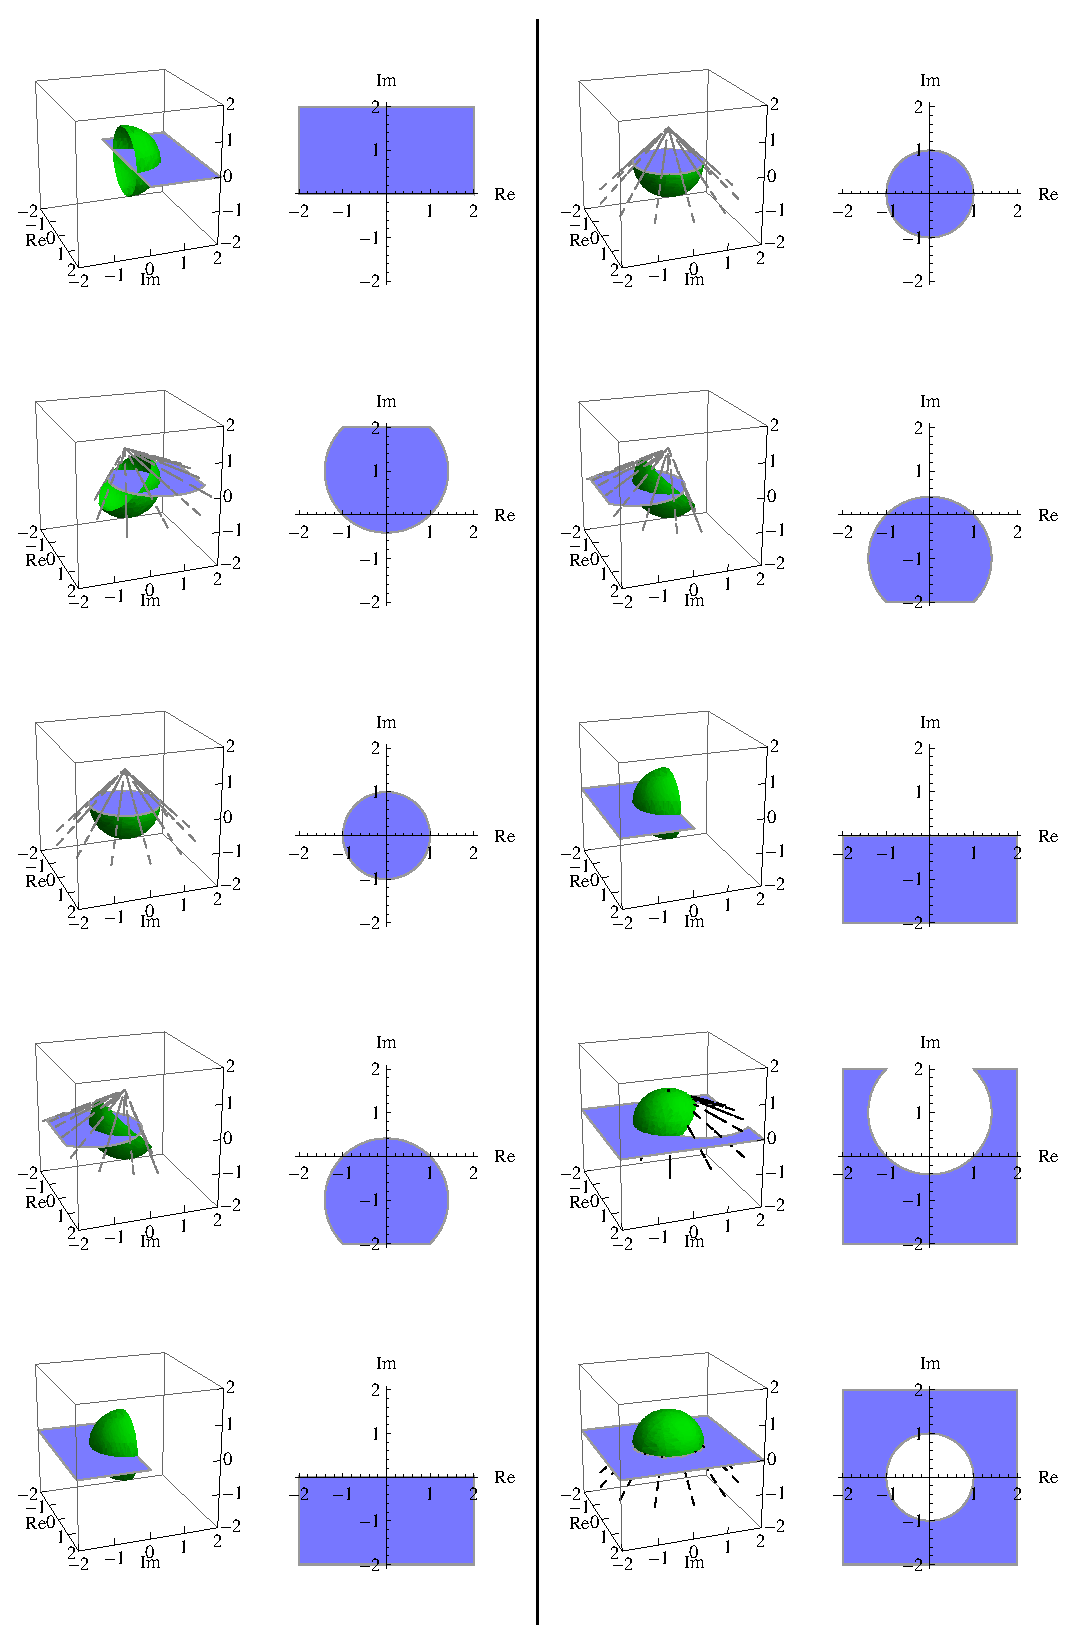
\includegraphics[width=0.9\textwidth]{figures/stereo-proj-1}
\caption[Stereographic projection and the map $z \mapsto \reci{z}$]{Inversion $z \mapsto \reci{z}$ can be interpreted as rotation of the Riemann sphere by $180^{\circ}$ around the $x_1$ axis. It maps the upper to the lower half-plane (left) and the interior of the unit circle to its exterior (right).}
\label{fig_StereoProjInversion}
\end{figure}

\begin{example}
\label{ex_StereoProjInversion}
Consider the map $f: z \mapsto \reci{z}$ and the map $V: \UnitSphere \to \UnitSphere$, which rotates the Riemann sphere around the $x_1$ axis by $180^{\circ}$:
\begin{equation}
\label{eqn_RiemannX1Rotation}
V: x \mapsto
\begin{pmatrix}
1 & \phantom{+}0 & \phantom{+}0 \\
0 & -1           & \phantom{+}0 \\
0 & \phantom{+}0 & -1
\end{pmatrix}
\cdot
\begin{pmatrix}x_1 \\ x_2 \\ x_3 \end{pmatrix}.
\end{equation}
The first row of Figure~\ref{fig_StereoProjInversion} shows the upper half-plane $U$ on the left and the unit disk $D$ on the right together with their images under reverse stereographic projection. We see that both, $U$ and $D$, correspond to a certain ``halfsphere'' of the Riemann sphere. If we rotate these halfspheres around the $x_1$ axis (leaving the points $\{\pm 1\}$ fixed) and continuously perform stereographic projection, we see that after a half turn (in the last row of Figure~\ref{fig_StereoProjInversion}) we end up with the lower half-plane $f(U)$ and the set of points $z$ with $\abs{z} > 1$, $f(D)$. 

It is worth noting that this correspondence between rotation of the Riemann sphere by $180^\circ$ and the map $f : z \mapsto \reci{z}$ does not just hold for the specially chosen sets $U$ and $D$, but indeed pointwise for every $z \in \EC$. In other words, we have
\begin{equation*}
f = P_{\UnitSphere} \circ V \circ P_{\UnitSphere}^{-1}.
\end{equation*}
We show this by a simple calculation, using the fact that $\reci{z} = \frac{\conj{z}}{\abs{z}^2}$ as well as (\ref{eqn_RevStdStereoProj}) and noting that for the case $z = \infty$ limits have to be introduced appropriately:
\begin{IEEEeqnarray*}{rCcCl}
(P_{\UnitSphere}^{-1} \circ f)(z)
&=& \reci{\reci{\abs{z}^2} + 1} 
\begin{pmatrix}
  2 \Re{\reci{z}} \\ 2 \Im{\reci{z}} \\ \reci{\abs{z}^2} - 1
\end{pmatrix}
&=& \frac{\abs{z}^2}{1 + \abs{z}^2}
\begin{pmatrix}
  2 \reci{\abs{z}^2} \Re{\conj{z}} \\
  2 \reci{\abs{z}^2} \Im{\conj{z}} \\
  \frac{1 - \abs{z}^2}{\abs{z}^2}
\end{pmatrix} 
\\
&=&\reci{\abs{z}^2 + 1}
\begin{pmatrix}
  \phantom{+}2 \Re{z} \\ -2 \Im{z} \\ -\abs{z}^2 + 1
\end{pmatrix}
&=&
(V \circ P_{\UnitSphere}^{-1})(z).
\end{IEEEeqnarray*}
\end{example}

\begin{remark}
\label{rem_TRotation}
Other examples for transformations corresponding to a half-turn of the Riemann sphere are $z \mapsto -z$ (rotation around the $x_3$ axis) and $T: z \mapsto -\reci{z}$ (rotation around the $x_2$ axis; as product of half turns around the $x_1$ and $x_3$ axes). $T$ is a function which maps the upper half-plane to itself and which will be important in the study of the modular group in Section~\ref{sec_ModularGroupGenRel}.  
\end{remark}

\begin{figure}
\centering
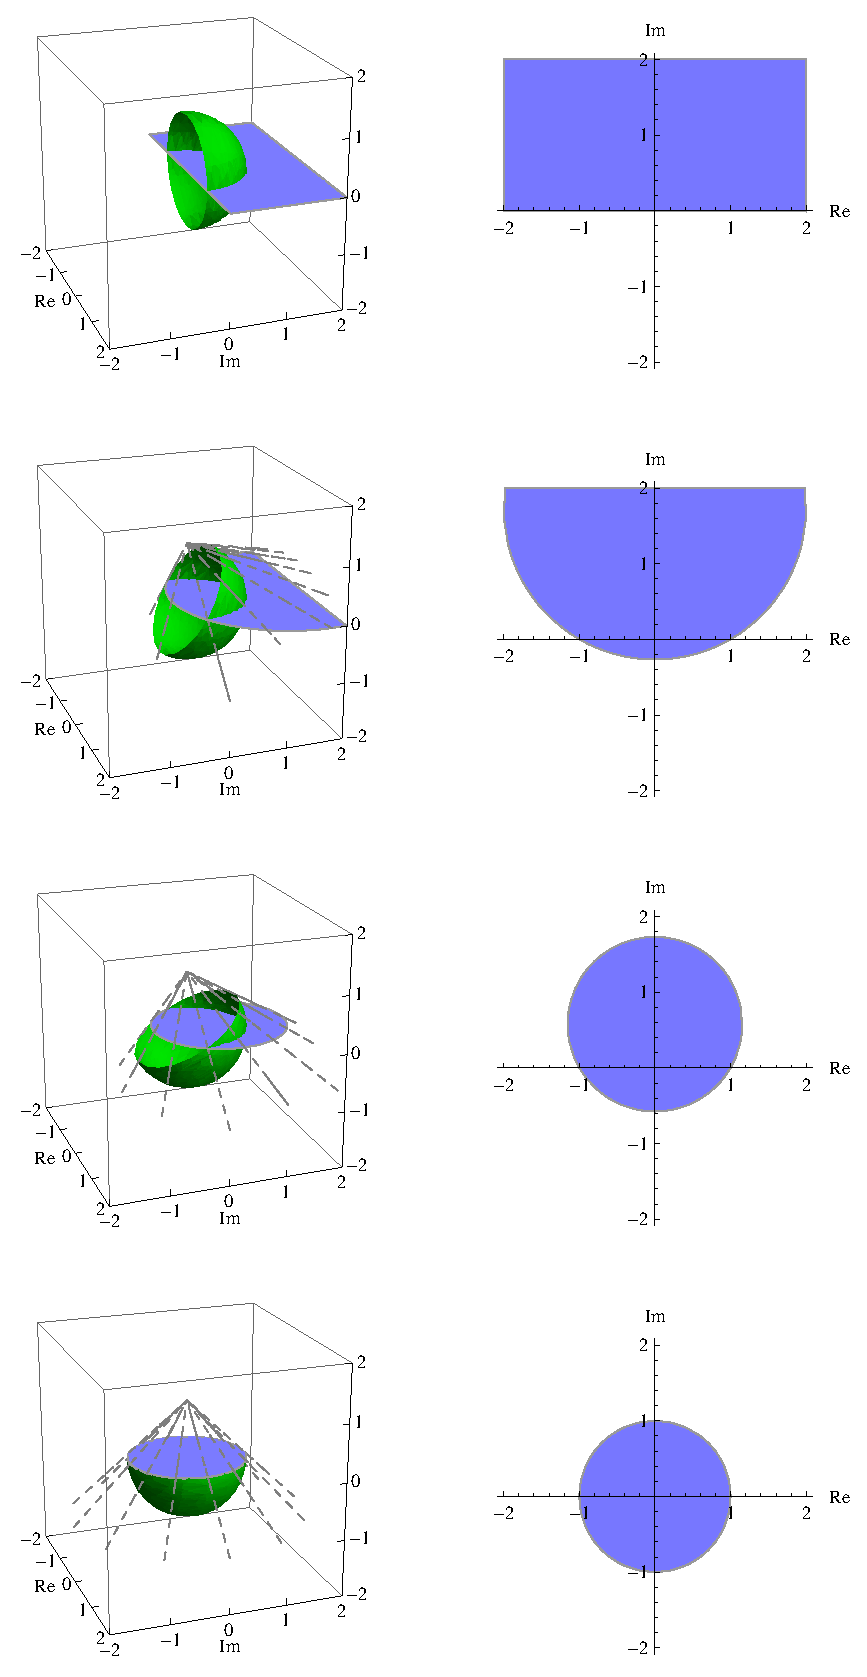
\includegraphics[width=0.7\textwidth]{figures/stereo-proj-2}
\caption[Stereographic projection and the modified Cayley transform]{The modified Cayley transform $z \mapsto \moebius{\ii}{1}{}{\ii}{z}$ maps the upper half-plane to the unit disk, leaving the points $\{\pm 1\}$ fixed. It can be considered as a quarter turn of the Riemann sphere around the $x_1$ axis.}
\label{fig_StereoProjModCayley}
\end{figure}

\begin{example}[Modified Cayley transform]
\label{ex_ModCayleyTransform}
\label{ex_StereoProjCayleyMap}
\index{Modified Cayley transform}
\index{Cayley transform}
In Figure~\ref{fig_StereoProjModCayley}, the action of yet another interesting transformation can be seen, which maps the upper half-plane to the unit disk. It is given by
\begin{equation}
\label{eqn_ModCayleyTransform}
\ModCayley(z) = \moebius{\ii}{1}{}{\ii}{z}
\end{equation}
and can be either considered as a quarter turn of the Riemann sphere around the $x_1$ axis or as ``half of an inversion'', since indeed $\ModCayley^2(z) = \ModCayley(\ModCayley(z)) = \reci{z}$ (compare with left column of Figure~\ref{fig_StereoProjInversion}). In contrast to its better known brother, the \emph{Cayley transform} given by
\begin{equation}
\label{eqn_CayleyTransform}
\Cayley(z) = \frac{z - \ii}{z + \ii} = -\ii \ModCayley(z),
\end{equation}
$\ModCayley$ leaves the points $\{\pm 1\}$ fixed, which often beneficial for visualization purposes. We will call $\ModCayley$ the \emph{modified Cayley transform}. 
\end{example}
\begin{remark} 
Also the Cayley transform $\Cayley$ can be seen as rotation of the Riemann sphere by $120^\circ$ around the axis which is spanned by the vector $(1,-1,1) \in \R^3$. A figure illustrating this fact can be found for example in \Mumford{}, p.\ 88.
\end{remark}

We have now seen exemplary that quite a few interesting maps are induced by rotations of the Riemann sphere. If we are willing to allow not only rotations but also translations of the Riemann sphere, we indeed obtain a new characterization of M�bius transformations, as stated in the next theorem.

\begin{definition}
\index{Rigid motion}
A \emph{rigid motion} of $\R^3$ is an affine transformation of $\R^3$ which is obtained purely by composition of rotations and translations.
\end{definition}

\begin{theorem}[M�bius transformations revealed]
\label{thm_MoebiusRevealed}
A function $\phi : \EC \to \EC$ is a M�bius transformation, if and only if it can be obtained by reverse stereographic projection of $\EC$ to an admissible sphere $S \subseteq \R^3$, followed by a rigid motion T of $\R^3$ which maps $S$ to another admissible sphere $TS$, followed by stereographic projection from $TS$ back to $\EC$:
\begin{equation}
\label{eqn_MoebiusRevealedForm}
\phi = P_{TS} \circ T \circ P_S^{-1}.
\end{equation}
\end{theorem}
\begin{proof}[Sketch of proof]
The fact that all maps of form ($\ref{eqn_MoebiusRevealedForm}$) are indeed M�bius transformations can be seen either by direct calculation or by the observation that $\phi$ corresponds to the map $P_S^{-1} \circ \phi \circ P_S = P_S^{-1} \circ P_{TS} \circ T$ from $S$ to itself. If we identify $S$ with the Riemann sphere, we can regard $\phi$ as a holomorphic automorphism of the Riemann sphere which is therefore a M�bius transformation.

\todo{31}{Literature reference}

It remains to show that every given transformation can indeed be realized in the form (\ref{eqn_MoebiusRevealedForm}). For this purpose, we first consider the four basic types of M�bius transformations:
\begin{description}
\item[Translation:] The map $z \mapsto z + \alpha,\ \alpha \in \C$ can be realized by choosing an arbitrary admissible sphere $S$ and setting $T = T_{\alpha}: x \mapsto x + \iota(\alpha)$, which simply translates $S$ in a direction parallel to the $x_3 = 0$ plane by $\iota(\alpha)$.
\item[Dilation:] The map $z \mapsto \rho z,\ \rho > 0$ can be obtained by choosing an arbitrary admissible sphere with north pole $n$ and setting $T = D_{\rho}: x \mapsto x + \left(0, 0, (\rho-1) n_3\right)$, which moves $S$ up- ($\rho > 1$)  or downwards ($\rho < 1$) in $x_3$ direction.
\item[Rotation:] The map $z \mapsto \epo{\ii \theta} z,\ \theta \in (-\pi, \pi]$ can be realized by choosing an arbitrary admissible sphere and setting 
\begin{equation*}
T = R_{\theta}: x \mapsto 
\begin{pmatrix}
\cos{\theta} & -\sin{\theta}            & 0\\
\sin{\theta} & \phantom{+}\cos{\theta}  & 0\\
0            & \phantom{+}0             & 1
\end{pmatrix}
\cdot
\begin{pmatrix}x_1 \\ x_2 \\ x_3 \end{pmatrix},
\end{equation*}
which rotates $S$ around the $x_3$ axis by an angle of $\theta$.
\item[Inversion:] We have seen in Example~\ref{ex_StereoProjInversion} that the map $z \mapsto \reci{z}$ can be realized by choosing $S$ as the unit sphere $\UnitSphere$ and setting $T = V$ -- as defined in (\ref{eqn_RiemannX1Rotation}) -- which is a rotation of $\UnitSphere$ around the $x_1$ axis by an angle of $180^{\circ}$.
\end{description}
Now let $\phi(z) = \moebius{a}{b}{c}{d}{z}$ be an arbitrary M�bius transformation. As in the proof of Lemma~\ref{lem_MoebiusGenerators}, if $c = 0$ we may assume without restriction that $d = 1$ and therefore $\phi(z) = az + b$. Clearly this map can be realized in the form (\ref{eqn_MoebiusRevealedForm}) by starting with an arbitrary admissible sphere $S$ and taking $T$ as the composition of rotation by $\arg(a)$, dilation by $\abs{a}$ (in either order), followed by translation by $b$:
\begin{equation*}
T := T_b \circ D_{\abs{a}} \circ R_{\arg(a)}.
\end{equation*}
If $c \ne 0$, we can scale the coefficients $a,b,c,d$ such that $c = 1$ and write $\phi$ in the form
\begin{equation*}
\phi(z) = a + \frac{b - ad}{z + d}.
\end{equation*}
Now we choose $S$ to be the sphere with unit radius centered at the point $\iota(-d)$ and we compose $T$ out of the following rigid motions: First, translation by $d$ transforms $S$ to the unit sphere $\UnitSphere$. Thus we can indeed apply $V$ as the second transformation in order to perform an inversion. Finally we apply rotation and dilation by the factor $b - ad$ followed by a translation by $a$:
\begin{equation*}
T := T_a \circ D_{\abs{b - ad}} \circ R_{\arg(b - ad)} \circ V \circ T_d. \qedhere
\end{equation*}
\end{proof}


% --------------------------------------------- Subsection: Generalized circles
\subsection{Generalized circles}

\index{Generalized!circle}
From the geometric point of view, M�bius transformations have the beautiful property that they preserve generalized circles. \emph{Generalized circles} are either circles (in the usual sense) or lines on the complex plane $\C$. They can also be thought of circles on the Riemann sphere (\ie the extended complex plane $\EC$ projected to the unit sphere $\UnitSphere$, see Remark~\ref{rem_RiemannSphere}), where lines on the complex plane stand in a one-to-one correspondence to circles through the point $\infty$ on the Riemann sphere. In order to give an exact definition, we first make the following considerations:

A circle with center $m \in \C$ and radius $r > 0$ can be described as the set of points $z \in \C$ for which
\begin{equation*}
\abs{z - m} = r.
\end{equation*}
This is obviously equivalent to
\begin{equation*}
\abs{z - m}^2 = (z - m) \conj{(z - m)} = r^2
\end{equation*}
and
\begin{equation}
\label{eqn_Circle}
z \conj{z} - m \conj{z} - \conj{m} z + m \conj{m} - r^2 = 0.
\end{equation}
The generalization comes into play if we multiply this last equation by a constant $A \in \R$
\begin{equation*}
A z \conj{z} - A m \conj{z} - A \conj{m} z + A m \conj{m} - A r^2 = 0
\end{equation*}
and introduce constants $B$, $C$ and $D$ appropriately such that we can write it in the form
\begin{equation}
\label{eqn_GenCircle}
A z \conj{z} + B \conj{z} + C z + D = 0.
\end{equation}
Note that $D$ is real and $B = \conj{C}$ are complex conjugates. From an equation of form (\ref{eqn_GenCircle}) we can read off the center and radius of the corresponding circle by
\begin{IEEEeqnarray}{rCl}
m &=& -\frac{B}{A}, \IEEEyessubnumber \\
r &=& \sqrt{m \conj{m} - \frac{D}{A}} = \sqrt{\frac{BC - AD}{A^2}}. \IEEEyessubnumber
\end{IEEEeqnarray}
Clearly we can only do so, if $A \ne 0$ and $BC - AD > 0$. 

In the case when $A = 0$, equation (\ref{eqn_GenCircle}) can be written as
\begin{equation*}
\Re{\frac{C}{\abs{C}} z} = -\frac{D}{2 \abs{C}},
\end{equation*}
which defines a line on the complex plane. We see this by considering the simpler equation $\Re{z} = -\frac{D}{2 \abs{C}}$ first (we omit the factor $\frac{C}{\abs{C}}$), which obviously defines a line parallel to the imaginary axis through the real point $-\frac{D}{2 \abs{C}}$. Then we observe that the multiplication with $\frac{C}{\abs{C}}$ just rotates this line clockwise around the origin by an angle which is given by $\arg(C)$.

To conclude our considerations, we note that equation (\ref{eqn_GenCircle}) can also be written in matrix form:
\begin{equation*}
\rvec{\conj{z}}{1} \cdot \mat{A}{B}{C}{D} \cdot \cvec{z}{1} = 0.
\end{equation*}
The matrix in this equation has a negative determinant, because of the condition $BC - AD > 0$ from above. Moreover, it is a Hermitian matrix, a notion which we will shortly recall:
\begin{definition}
\label{dfn_HermitianMatrix}
\index{Hermitian!matrix}
\index{Hermitian!transpose}
\index{Conjugate transpose}
Let $n > 0$ and $M \in \Mat{\C}{n}{n}$. The matrix
\begin{equation*}
\htransp{M} := \transp{\overline{M}}
\end{equation*}
obtained by complex conjugation and transposition of $M$ is called \emph{Hermitian transpose} or \emph{conjugate transpose} of $M$. If $M$ has the property $\htransp{M} = M$, it is called a \emph{Hermitian} matrix.
\end{definition}
Having now the right vocabulary at hand, we can give an exact definition for generalized circles.
\begin{definition}
Let $M = \smallmat{A}{B}{C}{D} \in \Mat{\C}{2}{2}$ be a Hermitian matrix with $\det(M) < 0$. A \emph{generalized circle} is the set of solutions $z \in \C$ to
\begin{equation}
\label{eqn_GenCircleMat}
\rvec{\conj{z}}{1} \cdot M \cdot \cvec{z}{1} = 0
\end{equation}
plus eventually the point $\infty$, if and only if $A = 0$, \ie when the generalized circle corresponds to a line on the complex plane.
\end{definition}

\begin{remark}
Since there should be no danger of confusion, we will from now on use the same name for a generalized circle and its corresponding Hermitian matrix (which is uniquely determined up to a real scalar factor).
\end{remark}

\begin{remark}
\label{rem_GeneralizedDisk}
\index{Generalized!disk}
One could easily do the same thing as above starting with the equations
\begin{equation*}
\abs{z - m} < r \quad \text{or} \quad  
\abs{z - m} \le r
\end{equation*}
instead of $\abs{z - m} = r$, which naturally leads to the notions of open or closed \emph{generalized disks}, determined by
\begin{equation}
\rvec{\conj{z}}{1} \cdot M \cdot \cvec{z}{1} < 0 \quad \text{or} \quad
\rvec{\conj{z}}{1} \cdot M \cdot \cvec{z}{1} \le 0.
\end{equation}
\end{remark}

\begin{theorem}
\label{thm_MoebiusGenCircle}
Let $M \in \Mat{\C}{2}{2}$ be a Hermitian matrix with $\det(M) < 0$ and $P \in \GL{\C}$. The image of the generalized circle $M$ under the M�bius transformation $\phi$ corresponding to the matrix $P \in \GL{\C}$ is the generalized circle  $\htransp{(\inv{P})} \cdot M \cdot \inv{P}$.
\end{theorem}
\begin{proof}
Let us write $P = \smallmat{a}{b}{c}{d}$, such that the corresponding M�bius transformation $\phi$ has the form
\begin{equation*}
\phi(z) = \moebius{a}{b}{c}{d}{z}.
\end{equation*}
Now we set $w = \phi(z)$ and show that 
\begin{equation*}
\rvec{\conj{z}}{1} \cdot M \cdot \cvec{z}{1} = 0
\end{equation*}
if and only if
\begin{equation*}
\rvec{\conj{w}}{1} \cdot \htransp{(\inv{P})} \cdot M \cdot \inv{P} \cdot \cvec{w}{1} = 0.
\end{equation*}
But this follows immediately from
\begin{equation*}
P \cdot \cvec{z}{1} = \cvec{a z + b}{c z + d} = (c z + d) \cvec{w}{1}.\qedhere
\end{equation*}
\end{proof}




% ----------------------------------------------------- CHAPTER: THEORETIC PART
\chapter{The modular group and its subgroups}

% ------------------------------------------------------ Section: Modular group
\section{The modular group}

Throughout this section and also later, we adopt the notation of Schoeneberg \cite{schoeneberg1974elliptic}.

\begin{definition}
\label{dfn_ModularGroup}
\index{Modular!group}
\index{Modular!transformation}
\index{Inhomogeneous!modular transformation}
A M�bius transformation $\phi$ of the form
\begin{equation*}
\phi(z) = \moebius{a}{b}{c}{d}{z},\quad a,b,c,d \in \Z,\quad ad - bc = 1
\end{equation*}
is called \emph{(inhomogeneous) modular transformation}.
\end{definition}

\begin{theorem}
\label{thm_ModularGroup}
\index{Modular!group}
The set of modular transformations forms a discrete subgroup of the group of M�bius transformations and can be identified with the projective special linear group $\PSL{\Z}$. This group is called the \emph{modular group} and is denoted by $\ModGrp$.
\end{theorem}
\begin{proof}
The proof is very similar to that of Theorem \ref{thm_MoebiusGroup}. The only thing which has to be changed is the homomorphism $\pi$ defined in (\ref{eqn_homPi}). Its domain now is $\SL{\Z}$, the group of 2-by-2 matrices over $\Z$ with determinant 1, rather than $\GL{\C}$ (or $\SL{\C}$). Again it follows by the first isomorphism theorem, that the modular group $\ModGrp$ is isomorphic to $\SL{\Z} / \ker(\pi) \cong \PSL{\Z}$. The fact that $\ModGrp$ is a discrete subgroup of the group of M�bius transformations is now also directly evident.
\end{proof}

\begin{remark}
\index{Inhomogeneous!modular transformation}
\index{Homogeneous!modular transformation}
\index{Modular!transformation}
The elements of $\SL{\Z}$ are often called \emph{homogeneous modular transformations}, whereas the transformations of $\ModGrp = \PSL{\Z}$ are called \emph{inhomogeneous}. Strictly seen, an inhomogeneous transformation has to be denoted as $[M]_{\sim}$, which is the equivalence class in $\PSL{\Z}$ of a matrix $M \in \SL{\Z}$. It is clear, that $[M]_{\sim}$ is nothing but the set $\{\pm M\}$ and again for easier notation, we will from now on simply write either $M$ or $-M$ instead of $[M]_{\sim}$.
\end{remark}

\todo{16}{Basic mapping properties}

\subsection{Generators and relations}

In group theory it is an important question, which systems of group elements and relations (in the sense of definition \ref{dfn_GrpConstructGenRel}) completely describe the structure of any given group. This section is devoted to the answer of this question in the case of the modular group.

Before we start, we introduce the following modular transformations which will serve as group generators:

\begin{IEEEeqnarray*}{RL}
U: & z \mapsto z + 1 \\
T: & z \mapsto -\reci{z} \\
R = TU: & z \mapsto -\reci{z + 1}
\end{IEEEeqnarray*}

\begin{remark}
Sadly, in literature there is no consensus about the notation of these transformations. We use the notation of Schoeneberg \cite{schoeneberg1974elliptic} here, but other notations are frequent. In Klein/Fricke \cite{klein1966vorlesungen}, the symbol $S$ is used instead of $U$ and in other literature as well as on Wikipedia, additionally the roles of $S$ and $T$ are swapped.
\end{remark}

\begin{theorem}
\label{thm_ModGrpGen}
The modular group is generated by the elements $U: z \mapsto z+1$ and $T: z \mapsto -\reci{z}$. 
\end{theorem}
\begin{proof}
Let $A: z \mapsto \moebius{a}{b}{c}{d}{z}$ be an arbitrary modular transformation. Our goal is to show that $A$ can be written as product of the transformations $U$ and $T$. For this purpose it is more convenient to view these transformations as elements of $\PSL{\Z}$, namely
\begin{equation*}
A = \mat{a}{b}{c}{d}, \quad U = \mat{1}{1}{0}{1}, \quad T = \mat{0}{-1}{1}{\phantom{+}0}.
\end{equation*}

Let's first consider the two special cases, when $a$ or $c$ are zero. If $a=0$, it follows from $ad - bc = 1$, that $-b = c = \pm 1$.  Therefore we have
\begin{equation*}
A \sim c A = \mat{0}{-1}{1}{c d} = TU^{c d}.
\end{equation*}
Similarly, $c = 0$ gives $a = d = \pm 1$ and
\begin{equation*}
A \sim a A = \mat{1}{a b}{0}{1} = U^{a b}.
\end{equation*}
In the general case, when $a$ and $c$ are both nonzero, $ad - bc = 1$ implies that $a$ and $c$ are coprime and the Euclidean algorithm therefore yields
\begin{eqnarray*}
      a &=& q_0 \cdot c\phantom{_0} + r_1 \\
      c &=& q_1 \cdot r_1 + r_2 \\
    r_1 &=& q_2 \cdot r_2 + r_3 \\
        &\vdots& \\
r_{n-1} &=& q_n \cdot r_n + r_{n+1}\\
        &=& q_n \cdot 1\phantom{_n} + 0.
\end{eqnarray*}
We can use this to reduce the Matrix $A$ by successively multiplying powers of $U$ and $T$ from the left. Just note, that multiplication with $U^k$ adds $k$ times the second row to the first row, whereas $T$ swaps the rows and changes the sign of one arbitrary row\footnote{This freedom of choice is again due to the fact that the matrices $M$ and $-M$ represent the same element in $\PSL{\Z}$.}. If we concentrate only on the first column of $A$ and apply the first few transformations
\begin{equation*}
\cvec{a}{c}                           \overset{U^{-q_0}}{\longmapsto}
\cvec{r_1}{c\phantom{_1}}             \overset{T}{\mapsto} 
\cvec{\phantom{+}c\phantom{_1}}{-r_1} \overset{U^{q_1}}{\longmapsto}
\cvec{\phantom{+}r_2}{-r_1}           \overset{T}{\mapsto} 
\cvec{r_1}{r_2}                       \overset{U^{-q_2}}{\longmapsto}
\cvec{r_3}{r_2}                       \overset{T}{\mapsto}
\cvec{\phantom{+}r_2}{-r_3}           \mapsto \dots,
\end{equation*}
we soon recognize the general mapping rule, which is
\begin{IEEEeqnarray*}{rCll}
\cvec{\phantom{+}r_{j-1}}{\phantom{+}r_{j\phantom{+0}}} 
& \overset{TU^{-q_j}}{\longmapsto}
& \cvec{\phantom{+}r_{j\phantom{+0}}}{-r_{j+1}}
& \quad \text{for even } j \text{ and}\\
\cvec{\phantom{+}r_{j-1}}{-r_{j\phantom{+0}}}
& \overset{TU^{q_j}}{\longmapsto}
& \cvec{\phantom{+}r_{j\phantom{+0}}}{\phantom{+}r_{j+1}} 
& \quad \text{for odd } j.
\end{IEEEeqnarray*}
When we set $r_{-1} := a$ and $r_0 := c$, this rule is true for $0 \le j \le n$. Obviously the described procedure ends with
\begin{equation*}
\cdots \overset{T}{\mapsto}
\cvec{\phantom{+}r_{n\phantom{+0}}}{\pm r_{n+1}} = \cvec{1}{0}.
\end{equation*} 
Because we know the first column of the resulting matrix and its determinant, which is 1, we can conclude that for some $k \in \Z$ it must have the form
\begin{equation*}
\mat{1}{k}{0}{1} = U^k.
\end{equation*}
By setting $e_n := (-1)^{n} q_n$, we therefore have 
\begin{equation*}
TU^{-e_n} TU^{-e_{n-1}} \cdots TU^{-e_1}TU^{-e_0} A = U^k
\end{equation*}
or equivalently,
\begin{equation*}
A = U^{e_0} TU^{e_1} \cdots TU^{e_{n-1}} TU^{e_n} T U^k,
\end{equation*}
which gives the desired representation of $A$ in terms of $U$ and $T$ in the case when $a$ and $c$ are both non-zero.
\end{proof}

It is worth formulating the algorithm used in the previous proof explicitly in the following corollary.
\begin{corollary}
\label{cor_ModGrpTUAlg}
An arbitrary modular transformation $A: z \mapsto \moebius{a}{b}{c}{d}{z}$ can be represented in terms of the transformations $U: z \mapsto z+1$ and $T : z \mapsto -\reci{z}$, by performing the following steps:
\begin{enumerate}
\item If $a = 0$, then $A = TU^{c d}$ and if $c = 0$, then $A = U^{a b}$ and we are done. Otherwise, continue with \ref{itm_ModGrpTUAlgStart}.
\item \label{itm_ModGrpTUAlgStart} Apply the Euclidean algorithm to $a$ and $c$ with the first division being $a = q_0 \cdot c + r_1$ ($q_0$ may be $\le 0$) and let $n$ be the number of the  last division (start counting from 0). Call the arising quotients $q_0,q_1,\dots,q_n$.
\item For $j \in \{0,1,\dots,n\}$ set $e_j := (-1)^j q_j$.
\item Calculate the matrix product $TU^{-e_n} TU^{-e_{n-1}} \cdots TU^{-e_1}TU^{-e_0} A$ and multiply by $\pm 1$ in order to obtain a representation with positive diagonal elements. Read off the right-upper entry and call it $k$.
\end{enumerate}
The transformation $A$ can now be written as
\begin{equation}
\label{eqn_ModGrpTUAlg}
A = U^{e_0} TU^{e_1} \cdots TU^{e_{n-1}} TU^{e_n} T U^k.
\end{equation}
\end{corollary}

We have seen that $U$ and $T$ generate the modular group, but it is not yet clear, which group words in $U$ and $T$ give the same modular transformations. For example, it is easy to see that $T^2 = 1$ and $(TU)^3 = 1$ are relations satisfied by $T$ and $U$. Before we can show, that these two relations are ``the only ones'', \ie all other relations can be derived from them, we need the following Lemma:

\begin{lemma}
Let $a, b, c, d \in \Z$ be arbitrary integers satisfying $ad - bc = 1$. Then one, and only one of the following three conditions is true:
\begin{IEEEeqnarray*}{RRCCCRCC}
  (i)\quad & ac       &\ge& 0 &\quad\land\quad&       bd &\ge& 0\\
 (ii)\quad & a^2 + ac &\le& 0 &\quad\land\quad& b^2 + bd &\le& 0\\
(iii)\quad & c^2 + ac &\le& 0 &\quad\land\quad& d^2 + bd &\le& 0
\end{IEEEeqnarray*}
\end{lemma}
\begin{proof}
It is trivial to see, that $(i)$ implies $\lnot (ii)$ and $\lnot (iii)$. It therefore remains to show, that $\lnot(i)$ implies either $(ii)$ or $(iii)$.
\end{proof}

\begin{theorem}
\label{thm_ModGrpRel}
The generators $T: z \mapsto -\reci{z}$ and $R: z \mapsto -\reci{z+1}$ of the modular group satisfy the relations
\begin{equation}
\label{eqn_ModGrpTRRel}
T^2 = \id{\C}, \quad R^3 = \id{\C}
\end{equation}
and all other relations are derived from these two. Therefore the modular group is isomorphic to the free product of a cyclic group of order 2 and a cyclic group of order 3.
\end{theorem}

\todo{18}{Proof}

% ------------------------------- Subsection: Fundamental domains, tessellation
\subsection{The fundamental domain and the tessellation of the halfplane}

\begin{figure}
\centering
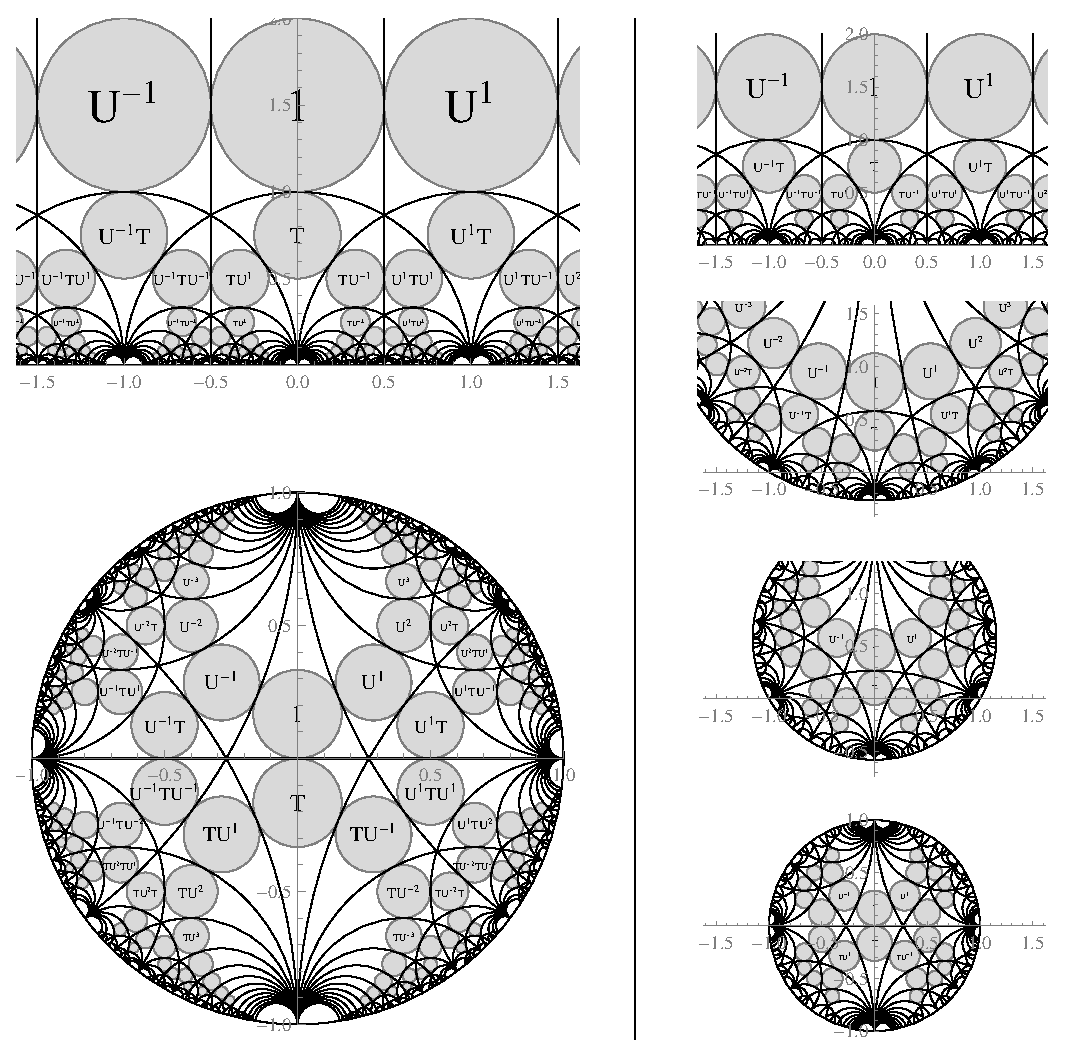
\includegraphics[width=\textwidth]{figures/modular-tiling-1}
\caption{The tessellation of the upper halfplane.}
\label{fig_ModularTiling}
\end{figure}


\todo{25}{Definition, description and figures}


% --------------------------------------------- Subsection: Hyperbolic geometry
\subsection{Hyperbolic geometry}

\todo{11}{Connection to hyperbolic geometry (disk/halplane model)}


% ------------------------------- Subsection: Ford circles, continued fractions
\subsection{Ford circles and continued fractions}

For an arbitrary modular transformation $A$, a representation as product of shifts $U^j: z \mapsto z+j$ and inversions $T: z \mapsto -\reci{z}$ can be found by the algorithm described in Corollary \ref{cor_ModGrpTUAlg}. By writing out this product, for example in the case when $n=2$, we have
\begin{equation*}
A = U^{e_0}T U^{e_1}T U^{e_2}T U^k,
\end{equation*}
or more explicitly
\begin{equation}
\label{eqn_ALongConFrac}
A(z) = e_0 - \reci{e_1 - \reci{e_2 - \reci{k + z}}}.
\end{equation}
\index{Continued fraction}
Here, a close relation between modular transformations and continued fractions immediately gets apparent. In this section we will investigate this relation somewhat deeper. 
First, we will use Pringsheim's more space-saving notation for continued fractions, namely
\begin{equation}
\label{eqn_ConFracNotation}
b_0 + \frac{a_1}{b_1 + \frac{a_2}{b_2 + \frac{a_3}{b_3 + \dots}}} =: 
b_0 + \cfr{a_1}{b_1} + \cfr{a_2}{b_2} + \cfr{a_2}{b_3} + \dots
\end{equation}
In the case when all $a_j = 1$, we adhere to the standard sequence notation for continued fractions:
\begin{equation*}
b_0 + \reci{b_1 + \reci{b_2 + \dots}} =: [b_0,b_1,b_2,\dots].
\end{equation*}
We can now reformulate Corollary \ref{cor_ModGrpTUAlg} in order to construct a continued fraction representation of any given modular transformation.

\begin{corollary}
An arbitrary modular transformation $A(z) = \moebius{a}{b}{c}{d}{z}$ can be written as continued fraction
\begin{equation}
\label{eqn_ModTransConFrac}
A(z) = [q_0,q_1,\dots,q_n,(-1)^{n+1}(k+z)]
\end{equation}
where the integers $n$, $q_0,q_1,\dots,q_n$ and $k$ are determined by the algorithm described in Corollary \ref{cor_ModGrpTUAlg}.
\end{corollary}
\begin{proof}
By using the continued fraction representation of $A$ given in (\ref{eqn_ALongConFrac}) and by applying the definition $e_j$ := $(-1)^j q_j$ we see
\begin{IEEEeqnarray}{rCcCcCcCcCcCc}
A(z) &=& e_0 &+& \cfr{-1}{e_1} 
          &+& \cfr{-1}{e_2} 
          &+& \dots 
          &+& \cfr{-1}{e_n} 
          &+& \cfr{-1}{k + z} \nonumber \\
  &=& q_0 &+& \cfr{-1}{-q_1} 
          &+& \cfr{-1}{q_2} 
          &+& \dots 
          &+& \cfr{-1}{(-1)^n q_n} 
          &+& \cfr{-1}{k + z}. \label{eqn_ModTransConFracInterim}
\end{IEEEeqnarray}
Now for every odd $j \le n$ we can rewrite 
\begin{equation*}
\cfr{-1}{-q_j} + \cfr{-1}{\dots} \quad \text{to} \quad \cfr{1}{q_j} + \cfr{1}{\dots}.
\end{equation*}
Thus if $n$ is odd, every numerator $-1$ in (\ref{eqn_ModTransConFracInterim}) can be turned into $+1$. In the other case, when $n$ is even, only one negative numerator at the end, $\frac{-1}{k+z}$, remains, but this can easily be rewritten to $\frac{1}{-(k+z)}$. Taking both cases together, we obtain (\ref{eqn_ModTransConFrac}).
\end{proof}

\begin{figure}
\centering
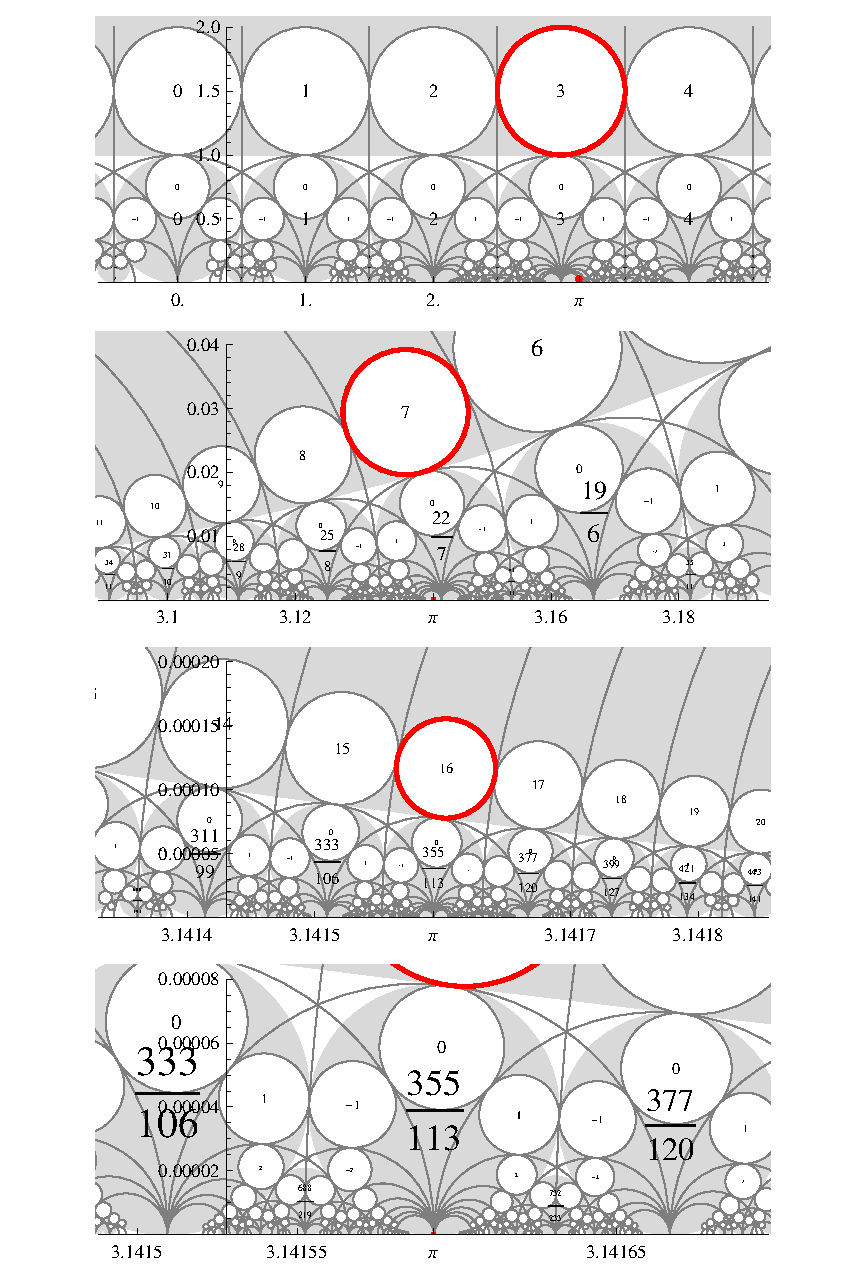
\includegraphics[width=\textwidth]{figures/cont-frac-pi}
\caption{$\pi = \frac{355}{113}$ -- well, almost.}
\label{fig_ContFracPi}
\end{figure}


\todo{19}{The modular group and ford circles}




% -------------------------------------------------- Section: Modular Subgroups
\section{Classical subgroups of the modular group}

\todo{24}{Subgroups of the modular group}


% --------------------------------------- CHAPTER: ALGORITHMS AND VISUALIZATION
\chapter{Algorithms and Visualization}

\todo{26}{More details on used algorithms for visualization}


\nocite{perron1913lehre}
\nocite{ford1938fractions}
\nocite{mumford2002indra}
\nocite{verrill2003fundamental}
\nocite{klein1966vorlesungen}

\printindex

\bibliographystyle{plain}
\bibliography{literature}

\end{document}
